% Created 2018-10-22 Mon 16:09
% Intended LaTeX compiler: pdflatex
\documentclass[11pt]{article}
\usepackage[utf8]{inputenc}
\usepackage[T1]{fontenc}
\usepackage{graphicx}
\usepackage{grffile}
\usepackage{longtable}
\usepackage{wrapfig}
\usepackage{rotating}
\usepackage[normalem]{ulem}
\usepackage{amsmath}
\usepackage{textcomp}
\usepackage{amssymb}
\usepackage{capt-of}
\usepackage{hyperref}
\date{\today}
\title{}
\hypersetup{
 pdfauthor={},
 pdftitle={},
 pdfkeywords={},
 pdfsubject={},
 pdfcreator={Emacs 26.1 (Org mode 9.1.14)}, 
 pdflang={English}}
\begin{document}

\tableofcontents

\section{Manuale di utilizzo della simbologia degli atti pianificatori del Canton Ticino per QGIS}
\label{sec:org21e8739}
La libreria comprendente la simbologia degli atti pianificatori del Canton
Ticino per QGIS (di seguito chiamata \emph{libreria}) è composta da:
\begin{itemize}
\item un file \texttt{libreria.xml} contenente la definizione di tutti i simboli
\item una directory contenente le immagini \texttt{svg} utilizzate nei simboli (327)
\end{itemize}
\subsection{Requisiti}
\label{sec:orgec07082}
La libreria è stata creata per essere compatibile con QGIS 2.18
\subsection{Installazione in QGIS}
\label{sec:org31e6c7c}
\subsubsection{SVG path}
\label{sec:org3ba5c3e}
Prima di importare la libreria \texttt{xml} è necessario configurare in QGIS dove si
trova la directory con le immagini. 
In \texttt{Impostazioni > Opzioni -> Sistema -> Percorsi SVG} è possibile aggiungere il percorso
della directory.
\begin{center}
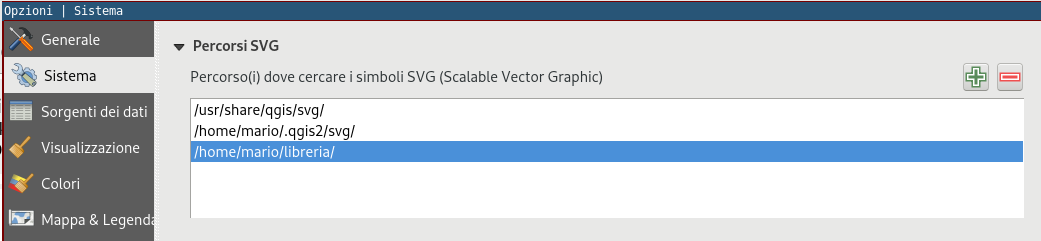
\includegraphics[width=.9\linewidth]{./path_svg.png}
\end{center}
\subsubsection{Import della libreria}
\label{sec:org6c48548}
Aprendo il gestore di stili dal menu \texttt{Impostazioni > Gestore di sili} è
possibile importare a scelta alcuni o tutti i simboli tramite il file \texttt{libreria.xml}
\begin{center}
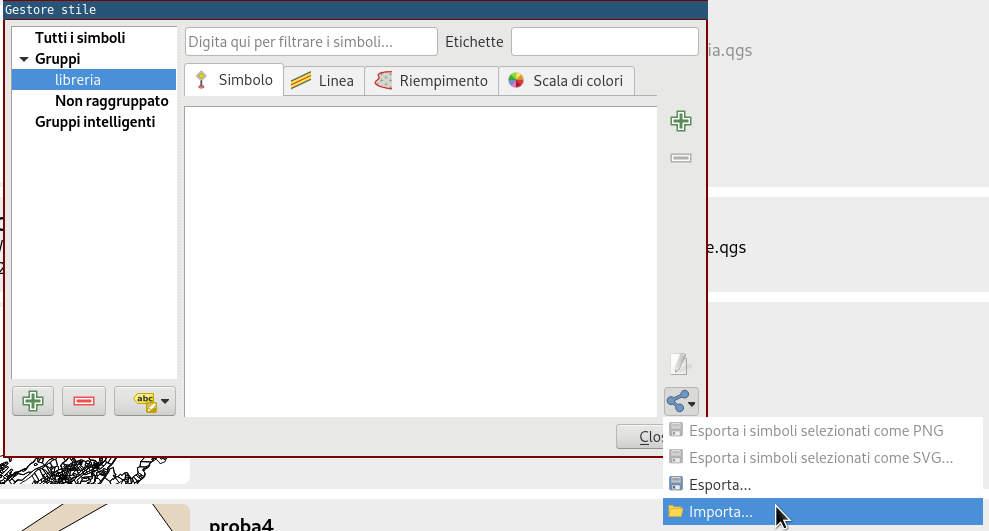
\includegraphics[width=.9\linewidth]{./import_xml.png}
\end{center}

\begin{center}
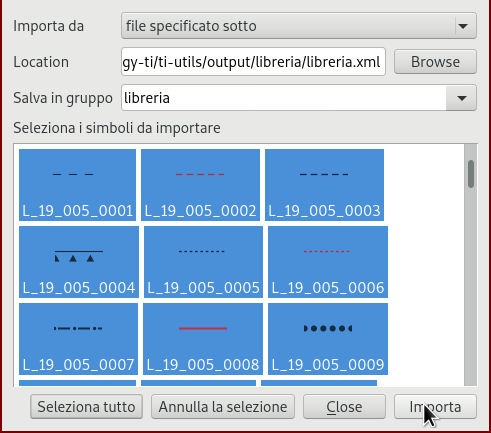
\includegraphics[width=.9\linewidth]{./import_symbols.png}
\end{center}
A questo punti i simboli sono pronti ad essere utilizzati.
\begin{center}
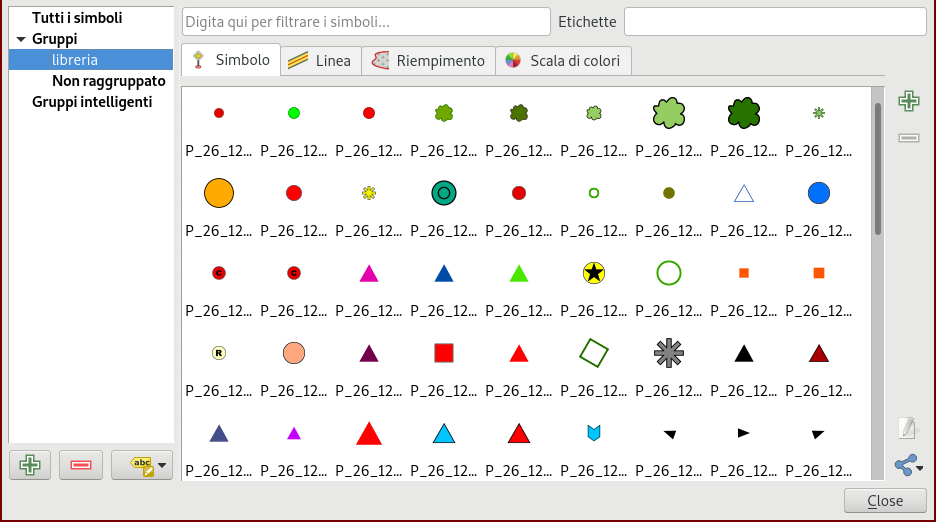
\includegraphics[width=.9\linewidth]{./imported_symbols.png}
\end{center}
\subsection{Possibili problemi}
\label{sec:org634e39f}
Nel caso venga importata la libreria senza che sia definito il percorso dei
file svg, oppure se la directory con i file svg viene spostata, i simboli che
utilizzano immagini svg appariranno come dei punti interrogativi. Per
risolvere il problema è sufficiente impostare il percorso correttamente e
riavviare QGIS. 
\end{document}
